\documentclass{article} \usepackage{tabularx}
\usepackage{amsmath} \usepackage{amssymb} \usepackage{tikz}
\usetikzlibrary{timeline} \usepackage{booktabs}
\usepackage{float} \restylefloat{table} \graphicspath{{images/}}
\usepackage[margin={3.5cm,3cm}]{geometry} \usepackage{multicol}
\setlength\columnsep{1.5cm} \usepackage{tabto}
\usepackage{pdflscape} \usepackage{graphicx} \usepackage{array}
\usepackage[T1]{fontenc} \usepackage[utf8]{inputenc}
\usepackage{charter} \usepackage{environ} \usepackage{tikz}
\usetikzlibrary{calc,matrix}
% For citations
\usepackage[sort,numbers]{StyFiles/natbib}
\renewcommand{\citename}{\citet} \renewcommand{\cite}{\citep}
\usepackage{StyFiles/natbibspacing}


% code by Andrew: http://tex.stackexchange.com/a/28452/13304
\makeatletter \let\matamp=& \catcode`\&=13 \makeatletter
\def&{\iftikz@is@matrix \pgfmatrixnextcell \else \matamp \fi}
\makeatother

\newcounter{lines} \def\endlr{\stepcounter{lines}\\}

\newcounter{vtml} \setcounter{vtml}{0}

\newif\ifvtimelinetitle \newif\ifvtimebottomline
\tikzset{description/.style={ column 2/.append style={#1} },
  timeline color/.store in=\vtmlcolor, timeline
  color=red!80!black, timeline color
  st/.style={fill=\vtmlcolor,draw=\vtmlcolor}, use timeline
  header/.is if=vtimelinetitle, use timeline header=false, add
  bottom line/.is if=vtimebottomline, add bottom line=false,
  timeline title/.store in=\vtimelinetitle, timeline title={},
  line offset/.store in=\lineoffset, line offset=4pt, }

\NewEnviron{vtimeline}[1][]{%
  \setcounter{lines}{1}%
  \stepcounter{vtml}%
  \begin{tikzpicture}[column 1/.style={anchor=east}, column
    2/.style={anchor=west}, text depth=0pt,text height=1ex, row
    sep=1ex, column sep=1em, #1 ]
    \matrix(vtimeline\thevtml)[matrix of nodes]{\BODY};
    \pgfmathtruncatemacro\endmtx{\thelines-1} \path[timeline
    color st] ($(vtimeline\thevtml-1-1.north
    east)!0.5!(vtimeline\thevtml-1-2.north west)$)--
    ($(vtimeline\thevtml-\endmtx-1.south
    east)!0.5!(vtimeline\thevtml-\endmtx-2.south west)$);
    \foreach \x in {1,...,\endmtx}{ \node[circle,timeline color
      st, inner sep=0.15pt, draw=white, thick]
      (vtimeline\thevtml-c-\x) at
      ($(vtimeline\thevtml-\x-1.east)!0.5!(vtimeline\thevtml-\x-2.west)$){};
      \draw[timeline color
      st](vtimeline\thevtml-c-\x.west)--++(-3pt,0); }
    \ifvtimelinetitle%
    \draw[timeline color
    st]([yshift=\lineoffset]vtimeline\thevtml.north west)--
    ([yshift=\lineoffset]vtimeline\thevtml.north east);
    \node[anchor=west,yshift=16pt,font=\large] at
    (vtimeline\thevtml-1-1.north west) {\textsc{Timeline
        \thevtml}: \textit{\vtimelinetitle}}; \else%
    \relax%
    \fi%
    \ifvtimebottomline%
    \draw[timeline color
    st]([yshift=-\lineoffset]vtimeline\thevtml.south west)--
    ([yshift=-\lineoffset]vtimeline\thevtml.south east); \else%
    \relax%
    \fi%
  \end{tikzpicture}
}

\begin{document}


\begin{titlepage}
	\centering
	\begin{figure}[H]
    \centering
    % \includegraphics[scale=0.5]{logo_nasa_trio_black@2x.png}
	\end{figure}
	\vspace{2cm} {\scshape\LARGE Ph.D. Research Proposal\par}
  \vspace{2cm}
  
  %%%%%%%%%%% Title
	{\scshape\LARGE

    Sequence Learning Using Deep Neural Networks With Flexibility
    \& Interpretability
    
    \par} {\huge\bfseries \par}
	
	\vspace{2cm} {\Large\itshape Chang \textsc{Li}\par} \vfill

  {\Large Supervisor\par} {\Large\itshape Prof. Dacheng
    \textsc{Tao}\par} \vfill

\end{titlepage}


\section{Aims \& Objectives}

\begin{enumerate}
\item Flexibility in modeling complex patterns with long-range
  dependencies
  \begin{enumerate}
  % DA-RNN
  \item Capturing complex non-linear correlations without prior
    knowledge and assumptions
  \item Encoding high dimensional input variables adaptively
  \item Discovering long term dependencies of encoded inputs
  % \item Novel insights in feature extraction of complex inputs
  % TODO: Capsule Net
  % TODO: Capsule's Equivalent Problem in RNN
  % \item Demonstrating both classification and regression problems
  \end{enumerate}
\item Network architectures with better computational properties
  % TODO: All you need is attention
\item Decoding/Encoding human intepretable representations
  from/into models
  % TODO: DARNN_Bilinear
  \begin{enumerate}
  \item Approximating deep neural networks' input-output
    relationships using human intepretable models
  \item Learning deep neural networks coupled with structured
    (potentially predefined) latent variable sequence
  \end{enumerate}
\end{enumerate}

\section{Synopsis}
\label{sec:synop}

This project is focused on investigating sequence data learning
using deep learning networks. We divide this project into three
phases. We first aim to solve long-term dependencies issues by
investigating RNNs based encoder-decoder models with attention
mechanism. Then we will try to generalize those algorithms into
broader network topologies such as CNNs and feed-forward networks
to achieve better computational performance. The last goal of
this project is to improve the interpretability of deep learning
networks by using conventional human friendly machine learning
techniques such as lasso regression, random forest and graphical
models.

\section{Background And Literature Review}
\label{sec:intro}

One interesting task in machine learning is modeling complex
sequences having long-term dependencies. Many applications such
as machine translation, complex dynamical system analysis,
activity recognition and behavioral phenotyping tools for
neuro-science involved with capturing non-linear patterns in
sequences. Sequence learning mainly have three difficulties:
approximating non-linear relationship among sequences, feature
selection and capturing long-term dependencies. Our primary aim
of this proposal is mainly focused on demonstrating those three
difficulties. 

Despite substantial effort has been made for modeling sequences,
many of those models are neither unable to approximate non-linear
relationships nor have rigid assumptions due to the dependency on
predefined form of prior function. For example, autoregressive
moving average (ARMA) model~\cite{hibon1997arma} and many of its
variants~\cite{brockwell2013time} have raised interests because
of their effectiveness in many real world applications. However,
those models cannot capturing non-linear relationships.
Probabilistic Graphical
Models~\cite{murphy2012machine,koller2009probabilistic} (PGM) are
very well studied for the past decades. With predefined prior
distributions from domain knowledge, PGMs are capable to encode
many sequence relationships such as Gaussian
Processes~\cite{frigola2014variational}, Hidden Markov
Models~\cite{eddy1996hidden} (HMM) and Linear Dynamic
Systems~\cite{bar1993estimation} (LDS). However, capabilities of
approximating non-linear patterns of PGMs are also severely
suffered from rigid assumptions over priors.

Deep Neural Networks~\cite{goodfellow2016deep} (DNNs) are
powerful and flexible models that have outperforming performance
on various difficult learning tasks such as image classification,
visual object recognition, machine translation and speech
recognition. With sufficient training data, DNNs usually can get
nice approximation of that information in a reasonable amount of
time~\cite{goodfellow2016deep}.

Despite the powerful capability of approximation, one significant
limitation of DNNs is that they require fixed dimension of inputs
and targets. \citename{sutskever2014sequence} in 2014
demonstrated this difficulty as sequence to sequence problems.
They introduced an encoder-decoder framework based on two
Recurrent Neural Networks (RNNs) and achieved a very successful
result in machine translation. The key ideas (as shown in
Figure~\ref{fig:en-de}) behind encoder-decoder networks and its
variants are that they first encode the whole sentence of words
into a single, fixed length variable using encoder network. Then
a decoder network is used to decode that variable and generate
translation. They enabled the network to take various length of
inputs by encoding each of them into a single and fixed length
variable. One major drawback is that ``indeed the performance of
a basic encoder–decoder deteriorates rapidly as the length of an
input sentence increases~\cite{attention}''. Since for many
sequence learning applications there exists many long-term
dependencies relationships, the question of solving this drawback
remains open.

\begin{figure}
  \centering
  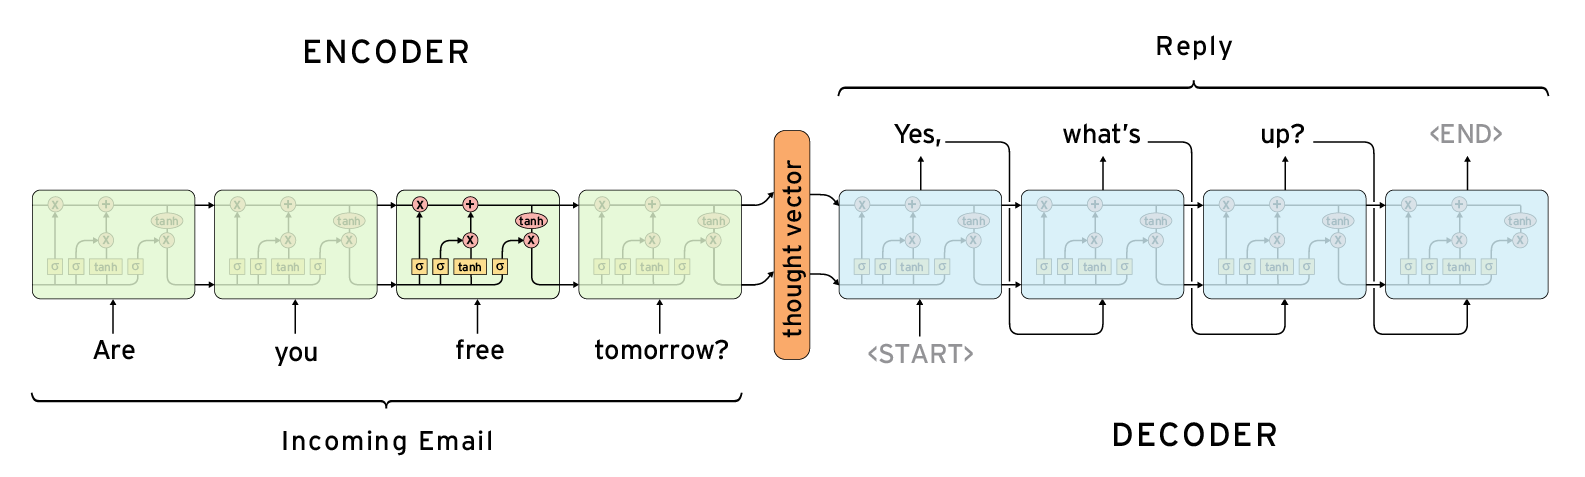
\includegraphics[scale=0.5]{images/en-de.png}
  \caption{Encoder-Decoder Network}
  \label{fig:en-de}
\end{figure}

Other than long-term dependencies difficulty, DNNs contain a very
large number of latent variables which make the training results
very hard for a human to interpret~\cite{goodfellow2016deep}.
Since DNNs are capable of approximating a very large number of
insignificant correlations between inputs and outputs of the
training data, there is no way to distinguish the true
relationships exist in data from suspicious correlations which
are caused by sampling bias in data
set~\cite{goodfellow2016deep}. Being able to explain the reasons
behind such models plays a crucial role in tasks such as model
comparison and deployment. It could also provide insights into
the data set and model itself. Thus improving the
interpretability of DNNs could also be a very interesting topic
to investigate.


\section{Proposed Methodology}
\label{sec:method}

We divide this project into three phases.

To commence we will investigate the mechanism of long-term
dependencies in time-series and how to model them using deep
neural networks. We will also investigate optimization algorithms
which can jointly optimize neural networks together with feature
selection.

With optimization algorithms in hand, at the second stage we will
try to extend those algorithms into various network topologies
such as CNNs and simple feed-forward neural networks. The goal of
the second stage is to investigate novel network topologies which
can preserve good approximation performance while having better
computational properties, such as parallelization.

At the final stage, we will explore a large group of conventional
machine learning methods (lasso regression, random forest,
graphical model, etc.) aiming at explaining the learning results
of neural networks. Outcomes at this stage not only improves the
interpretability of neural networks but also give insights on how
to encode expert prior knowledge into neural networks.

\subsection{Modeling Long-term Dependencies And Feature
  Selection}
\label{sec:ltfs}

As discussed in section~\ref{sec:intro}, encoder-decoder networks
based on RNNs outperform many other statistical machine learning
models while suffering from short-term memories due to encoding
global information into a single fixed length variable. One of
the most popular ways is to introduce ``attention mechanism''
into encoder-decoder networks~\cite{attention}.

\citename{attention} demonstrated long-term dependencies issue by
introducing context vectors in the middle of encoder network and
decoder network (as shown in Figure~\ref{fig:attention}). Instead
of encoding the global information into a single variable,
attention mechanism enables encoder network to provide a sequence
of encoded vectors on which decoder network can do soft-searches.
As a result, decoder network is able to concentrate on the most
relevant information represented by a subset of encoded vectors
of arbitrary length. Thus encoder-decoder networks can have much
better performance when dealing with long-term dependencies.

\citename{qin2017dual} extended \citename{attention}'s work to
adaptively select most relevant hidden states as well as most
significant features simultaneously. The developed a dual stage
RNNs (see Figure~\ref{fig:darnn}). Other than attention vector
between encoder and decoder layer (so called ``Temporal attention
Layer'' in Figure~\ref{fig:darnn}(b)), they adaptively weights
input sequence $x_t^k$ which is the $k$th feature at $t$ step by
attention $\alpha_t^k$ (see Figure~\ref{fig:darnn}(a)). The input
attention mechanism is a feed-forward network. Thus the extended
encoder-decoder network can weight features according to their
importance while the whole network can still be trained jointly.
However, their work is focused on regression. We will further
investigate their methods by extending to classification cases.

\begin{figure}
  \centering
  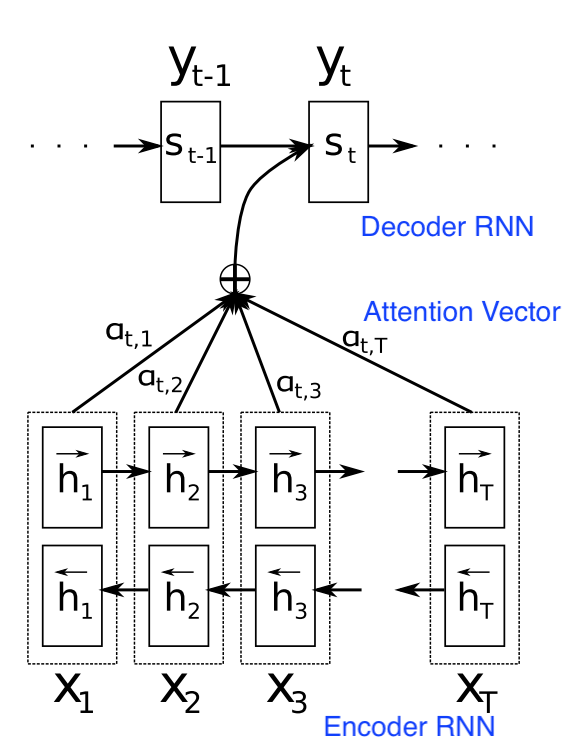
\includegraphics[scale=0.5]{images/attention.png}
  \caption{Attention Mechanism}
  \label{fig:attention}
\end{figure}

\begin{figure}[H]
  \centering
  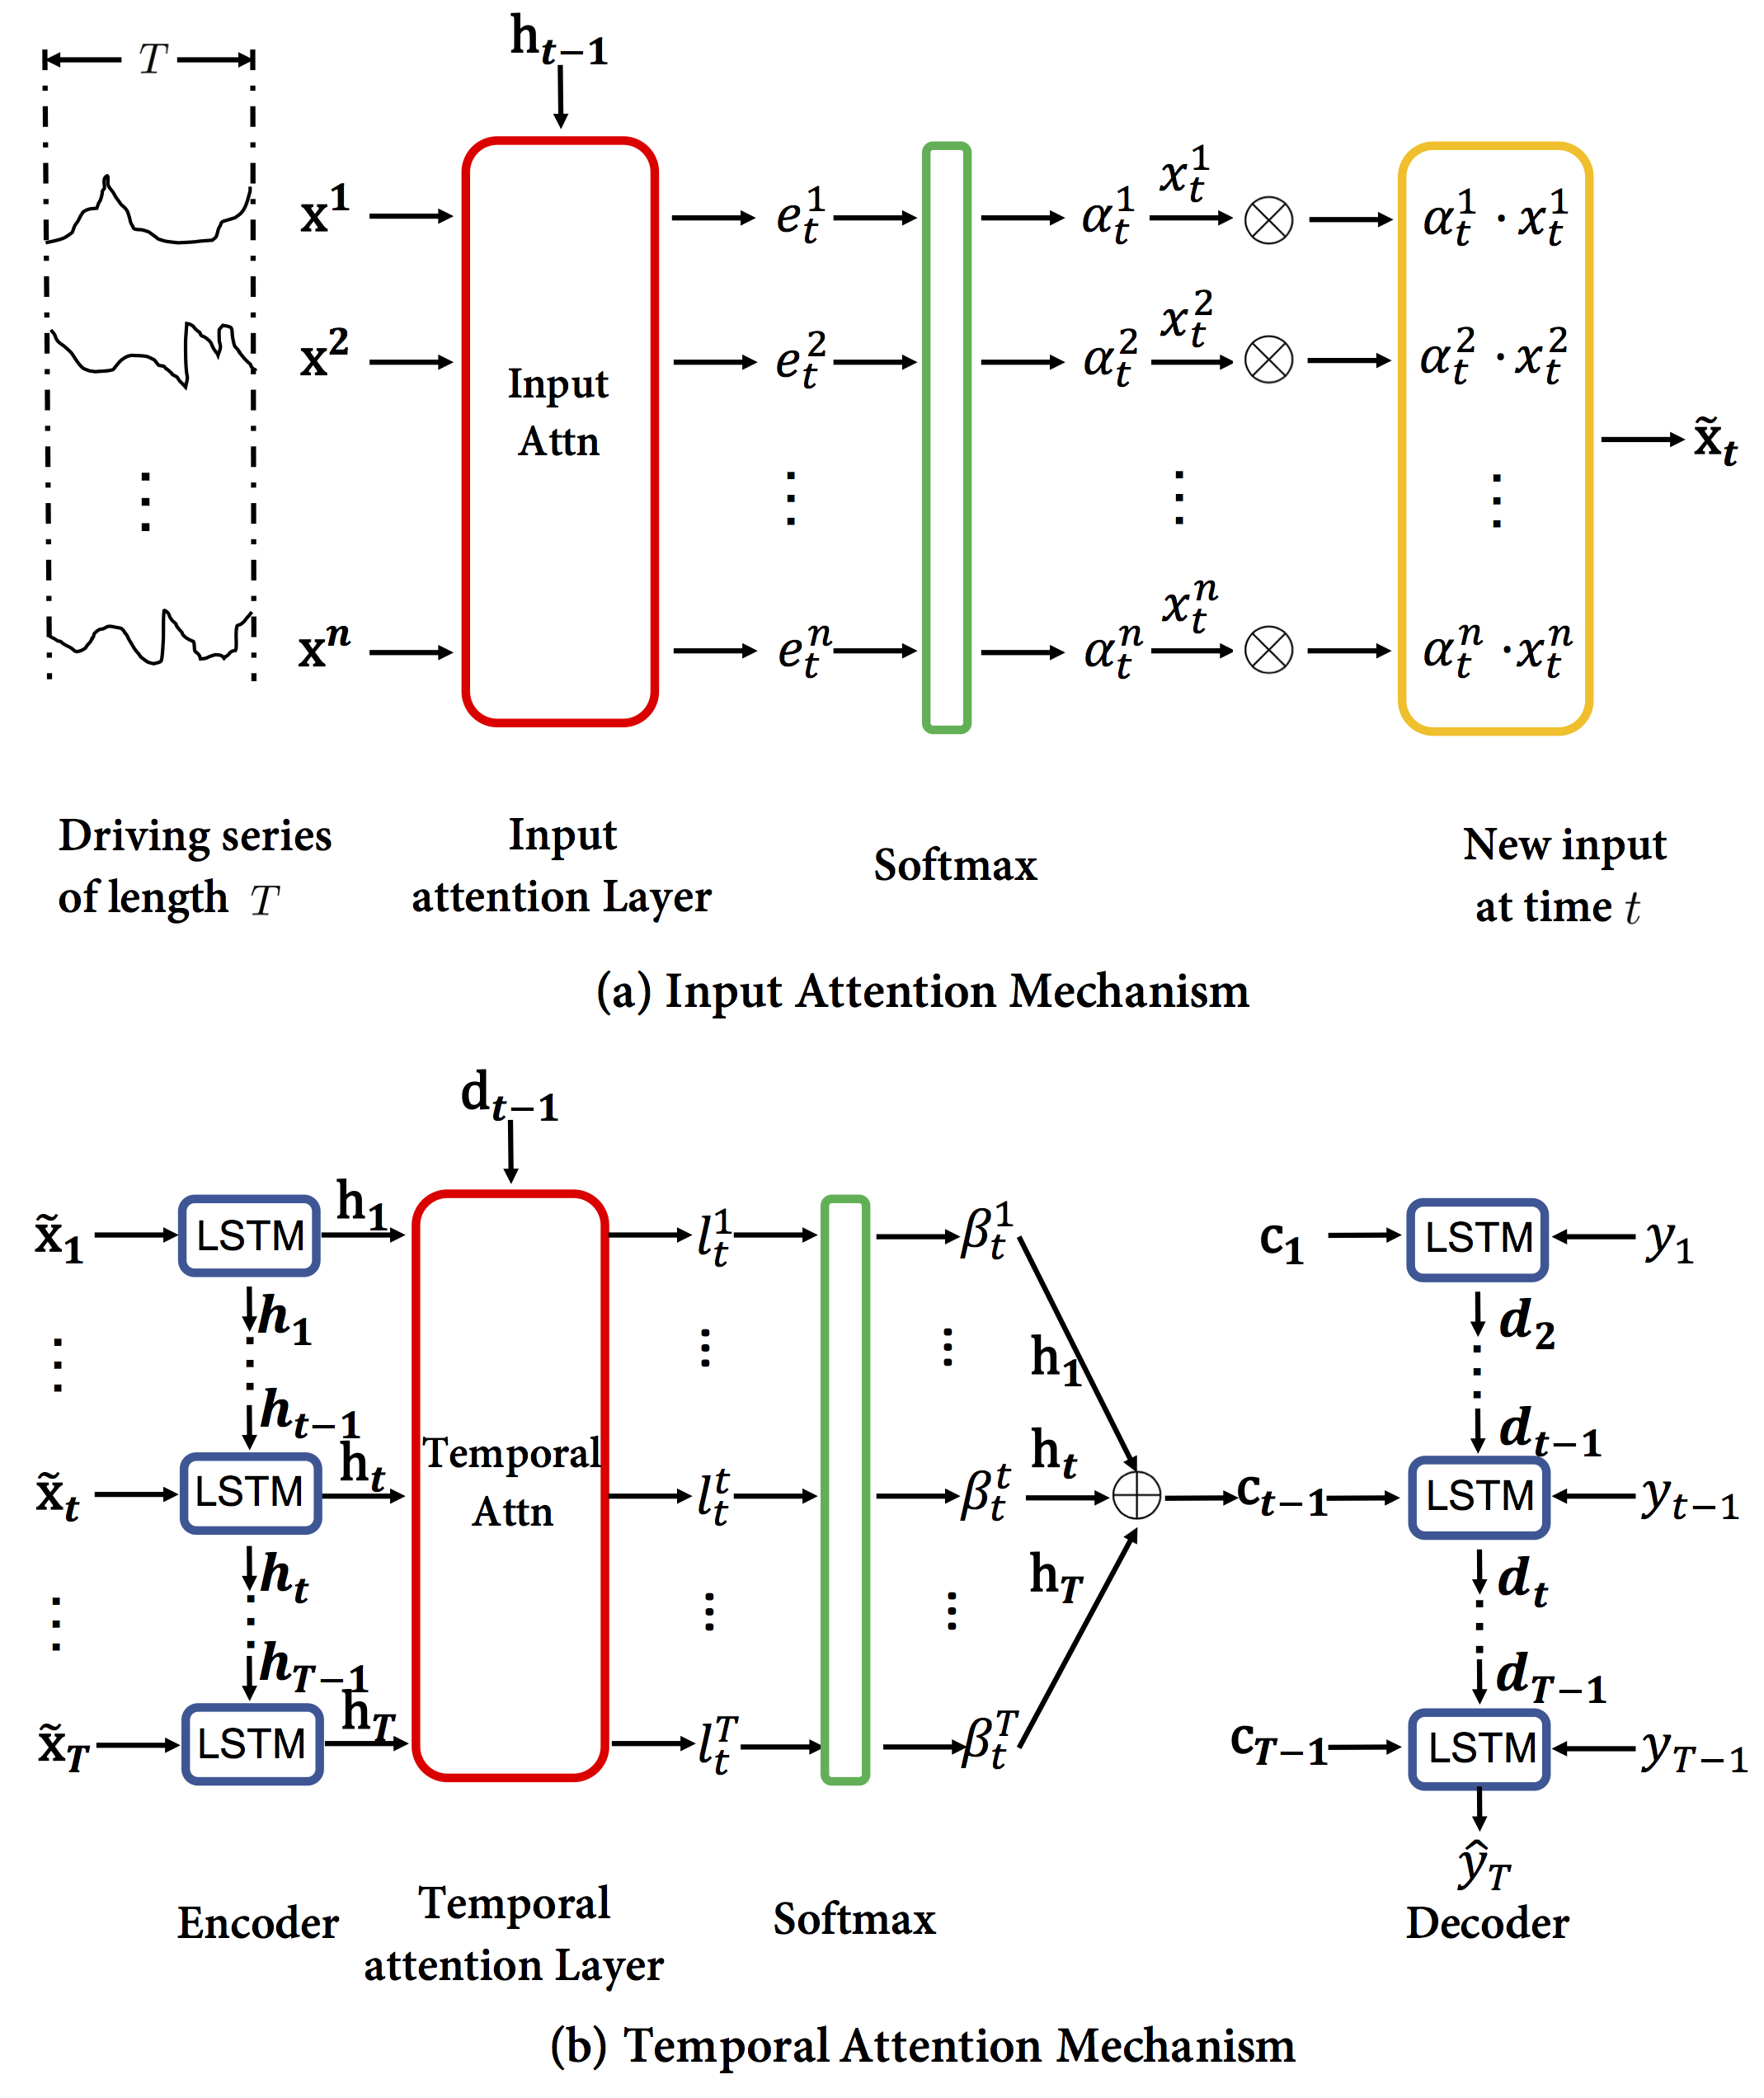
\includegraphics[scale=0.3]{images/darnn.png}
  \caption{Dual-Stage Attention Based RNN}
  \label{fig:darnn}
\end{figure}

\subsection{Topologies With Better Computational Properties}
\label{sec:better_comp}

One major drawback of RNNs formulation is computationally
expensive. RNNs usually have a very deep recursive structure. It
maintains hidden states of the entire past which prevents
parallel implementation of the algorithm. On the contrary,
Convolutional Neural Networks (CNNs) have a hierarchical
structure and can fully exploit the GPU hardware by using
parallel computing techniques.
\citename{gehring2017convolutional} attempted to replace RNNs
with CNNs in sequence modeling task by using a hierarchical
structure CNNs. They captured correlations in length of $n$
sequence by applying $\mathcal{O}(\frac{n}{k})$ convolutional
operations for kernels of width $k$ and constructed both of
encoder and decoder networks using CNNs. Results of their model
are slightly better than conventional encoder-decoder
networks~\cite{attention} on multiple data set but with a huge
decreasing in training time.

Recently, numerous pure attention architecture have been proposed
and achieved the state-of-the-art results in natural language
processing problems. \citename{vaswani2017attention} dispensed
CNNs and RNNs entirely and proposed a self-attention-based model.
They extends the conventional attention mechanism to a so-called
Multi-Head Attention (MHA) architecture by allowing each head to
generate different distributions over encoder output. This novel
network architecture has very concise topology representation and
outperforms both RNNs and CNNs based sequence to
sequence~\cite{vaswani2017attention}.

In this project we plan to further investigate those network
topologies. Besides, the question of creating attention mechanism
in input layers (feature selection) in those architectures still
remains open.

\subsection{Interpretability}
\label{sec:interp}

Substantial effort has been made for improving DNNs
interpretability in recent years. There are mainly three
different types of approaches:

\begin{itemize}
\item Explain local predictions directly
\item Approximating DNNs using human interpretative models
\item Joint learning probabilistic graphical models with DNNs
\end{itemize}

\citename{ribeiro2016should} proposed a Local Interpretative
Model-agnostic Explanations (LIME) method to interpret arbitrary
machine learning models directly by explain individual outputs.
They tried to approximate a human interpretative local estimator
(Lasso in their case) by sampling around models' outputs and
explain the reason behind those decisions by observing which
features (input) are taking most responsibility in the local
estimator. However, such approaches are limited to providing
explanations for individual decision. A more challenging task
would be providing a global insights of models.

Instead of explaining local predictions, \citename{SDT} use the
DNNs to train a soft decision tree. One main difficulty of such
model is that it requires exponentially large amount of training
data with respect to the depth of the tree. However, with
approximated DNNs in hand, sufficient amount of training data for
soft decision tree can be provided by labeling unlabeled data
using DNNs, sampling synthetic unlabeled data using generative
approach~\cite{goodfellow2014generative} and distilling
method~\cite{hinton2015distilling}. Such soft decision tree could
approximate DNNs to a reasonable extent while maintain human
interpretability for further investigation.

More advanced approaches combines complementary strengths of
Probabilistic Graphical Models (PGMs) and DNNs. As discussed
above, PGMs have very easy to understand structures. Other than
interpretability, they are also easy to fit and data efficient.
The main drawbacks of PGMs is that the rigid assumptions severely
limit PGMs capability of approximating non-linear relationship.
On the contrary, DNNs are highly capable of approximation while
are data intensive and hard to explain.
\citename{johnson2016composing} proposed a combination of
flexible deep learning feature models with structured Bayesian
priors. They used deep auto-encoders to extract lower
representation of non-linear observed data and used graphical
models for latent variables sequence inference. A very efficient
variational inference algorithm was developed to solve the joint
learning problem. A very interesting view of their work is that
other than providing better explanations, they also encoded human
expert knowledge into DNNs through
PGMs~\cite{johnson2016composing}. Investigation in this topic
could provide very interesting insights for both DNNs and PGMs
researches.

\section{Work Plan}

	\begin{table}[H]
		\centering
		\label{tab:work_plan}
		\def\arraystretch{1.5}%  1 is the default, change whatever you need
		\begin{tabularx}{\textwidth}{|X|l|}
			\hline
			\multicolumn{1}{|c|}{\textbf{Key Item}}                                                        & \multicolumn{1}{c|}{\textbf{Date}} \\ \hline
			Literature review and refine the scope of the project.
                                                                                                     &
                                                                                                       \multicolumn{1}{c|}{March
                                                                                                       -
                                                                                                       June
                                                                                                       2017}
      \\ \hline
			Re-implement models in section~\ref{sec:ltfs} and section~\ref{sec:better_comp} &
                                                                                        \multicolumn{1}{c|}{July
                                                                                        -
                                                                                        December
                                                                                        2017}            \\ \hline
			Implement feature selection mechanism for models in
      section~\ref{sec:better_comp} & \multicolumn{1}{c|}{January
                                      - April 2018}          \\ \hline
			Explore various topologies to achieve better computational
      performance & \multicolumn{1}{c|}{May - September 2018}             \\ \hline
			Write up experiment results for conference paper & \multicolumn{1}{c|}{September - December 2018}       \\ \hline
			Re-implement models in section~\ref{sec:interp} &
                                                        \multicolumn{1}{c|}{January
                                                        - April 2019}            \\ \hline
      Investigating explanations of previous models &
                                                      \multicolumn{1}{c|}{May - June 2019}                \\ \hline
			Write up experiment results for conference paper &
                                                         \multicolumn{1}{c|}{July - October 2019}                \\ \hline
			Write up thesis & \multicolumn{1}{c|}{November - January 2020}         \\ \hline
			Draft submission of thesis to supervisor and rework based on feedback                          & \multicolumn{1}{c|}{Early February 2020}              \\ \hline
			Thesis presentation/defense and submission to assessors. Potentially rework based on feedback  & \multicolumn{1}{c|}{March 2020}      		     \\ \hline
			Final submission of thesis                                                                     & \multicolumn{1}{c|}{April 2020}		             \\ \hline
		\end{tabularx}
		\caption{Estimated work plan}
	\end{table}

	
\bibliographystyle{abbrvnat} \bibliography{proposal.bib}
\end{document}
